\chapter{Testes de simulação} \label{cap:cap5}

Foram feitas avaliações das sensações proporcionadas pelo háptico como parte do projeto aprovado no comitê de ética do Hospital Universitário Antônio Pedro associado a faculdade de medicina da Universidade Federal Fluminense. Este projeto foi registrado na Plataforma Brasil do ministério da saúde sob o número 23637019.5.0000.5243 (texto no apêndice \ref{apend:comiteEtica}). A descrição destes experimentos e discussão dos resultados obtidos foram publicados em conferência da área \cite{Melo2021}.

Os experimentos foram apresentados a doze voluntários que fizeram uso do equipamento háptico, todos estes voluntários eram estudantes de ciência da computação com idades variando entre 18 e 44 anos sendo onze homens e uma mulher. Todos os voluntários concordaram com o termo de consentimento de participação nesta pesquisa (este está presente no apêndice \ref{apend:termoConsentimento}). Todos receberam uma breve explicação (cinco minutos) a respeito do procedimento de uso do equipamento háptico no experimento. Em seguida tiveram outros cinco minutos de tempo para usar um aplicativo de exemplo (para adquirir conhecimento sobre como interagir num ambiente com este tipo de dispositivo) visando nivelar o conhecimento.

Conforme comentado na seção anterior utilizamos o \textit{Haptic Plug-In For Unity3D} para programação das interações com o háptico utilizando o motor de jogo da \textit{Unity} \cite{UnityTechnologies2020} que é uma ferramenta muito utilizada para desenvolvimento de videogames e simulações com e sem \acrshort{RV} para diversas plataformas.
Este \textit{plugin} possibilita a interação do usuário com os objetos no ambiente virtual  de quatro modos distintos \cite{Poyade2014}. Para este experimento utilizamos o modo \textit{Puncture} (modo de punção) pelo requisito do experimento em simular uma agulha sendo inserida através de camadas representativas de tecidos.

O \textit{OpenHaptics driver} possui a definição de um conjunto de propriedades que representam como qualquer objeto 3D (camada, superfície, etc) tocável do ambiente virtual desenvolvido reage a cada interação com o dispositivo háptico. As propriedade mais relevantes no contexto do modo de punção são \textit{Stiffness}, \textit{Pop Through}, \textit{Static Friction}, e \textit{Dynamic Friction}. Todas elas têm como domínio um número real e aceitam valores entre zero e um. 

\textit{Stiffness} representa o nível de dureza do objeto: zero (0) representa um objeto mole e um (1) o objeto mais duro possível \cite{3DSystemsTouch2018}. Neste ponto é importante ressaltar que a quantidade de força máxima suportada depende das especificações do dispositivo háptico usado, dispositivos mais simples e de custo mais baixo comumente suportam intensidades de forças menores se comparadas a dispositivos mais complexos e com custos mais altos. \textit{Pop Through} controla o nível de força necessária para perfurar um objeto: zero indica que o objeto não pode ser perfurado e um que o máximo de força é necessário para perfurar o objeto \cite{3DSystemsTouch2018}. \textit{Punctured Static Friction} configura a dificuldade de se mover dentro de um objeto perfurado a partir de uma posição estática. O limite inferior (zero) representa um movimento sem atrito e o limite superior (um) representa a quantidade maior de atrito suportada pelo dispositivo \cite{3DSystemsTouch2018}. \textit{Punctured Dynamic Friction} controla a dificuldade de se mover dentro de um objeto depois que o movimento já foi iniciado \cite{3DSystemsTouch2018}. Da mesma forma que no caso estático o zero representa um movimento sem atrito e um o máximo de atrito suportado. Essas propriedades podem ser usadas para configurar o comportamento de cada camada de forma que o usuário tenha um experiência tátil de interação virtual que simule o procedimento real. As propriedades \textit{Stiffness} e \textit{Pop Through} precisam ser configuradas pra se determinar a força necessária por parte do usuário para perfurar cada objeto enquanto para determinar a força necessária para movimentação de uma agulha dentro de um objeto as propriedade a serem configuradas são \textit{Punctured Static Friction} e \textit{Punctured Dynamic Friction}.

Dois experimentos foram construídos para simular as diferentes sensações que os anestesistas experimentam enquanto executam punções lombares. Nestes experimentos os objetos 3D usados para simular as camadas do corpo foram simplificados e representados como hexaedros. Essa abordagem foi utilizada por que o objetivo destes experimentos era somente a avaliação das sensações de perfuração e deslocamento nas diferentes camadas proporcionadas pelo háptico e não algum tipo de avaliação estética. Deste modo foi removido o modelo 3D já desenvolvido para o simulador e foram utilizados modelos simplificados que não desviassem a atenção dos usuários do foco da avaliação. 
A Figura \ref{fig:visualExperimentos1e2} ilustra a forma que demonstramos visualmente os experimentos com elementos 3D com textura e sem transparência. Isto foi feito para que a resposta fosse somente de acordo com o retorno tátil obtido na mão do usuário ao usar o háptico sem dicas visuais a não ser o deslocamento da agulha. Incluímos um campo que demonstrava o deslocamento (profundidade) da agulha desde o início da perfuração pois algumas perguntas que formulamos nos experimentos dependiam do conhecimento destas distâncias entre o ponto de perfuração e cada uma das sensações. O usuário movimenta o elemento 3D que representa a agulha através do dispositivo háptico. Incluímos uma visão lateral a direita para que fosse possível observar a agulha e os objetos sendo perfurados de perfil. Desta forma foi possível observar facilmente quando a agulha estava totalmente inserida no objeto em cada experimento.
As imagens dos detalhes dos objetos 3D dos dois experimentos podem ser visualizados na Figura \ref{fig:objectsExperiments}. As setas de diferentes tamanhos no eixo Z ilustram as diferenças nos objetos 3D de cada experimento. A primeira camada (mais externa) é um cubo, e as demais camadas tem profundidades menores mas todas tem a mesma largura (eixo X) e altura (eixo Y), como pode ser visto na Figura \ref{fig:objectsExperiments}.

\begin{figure}[ht!]
    \centering
    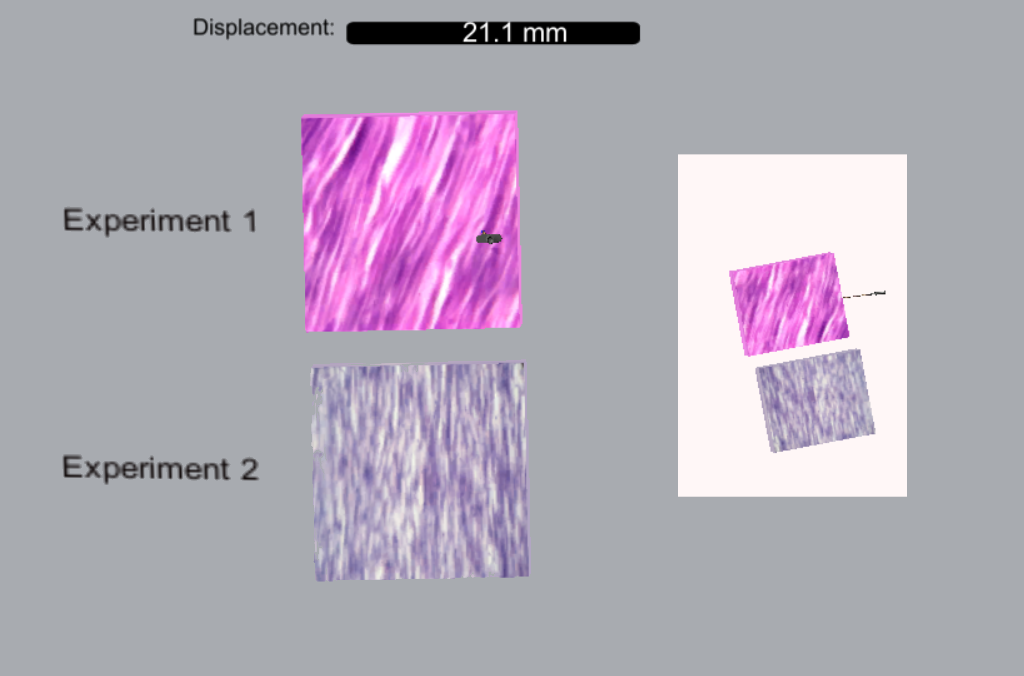
\includegraphics[width=0.8\linewidth]{capitulos/figuras/visual-experimentos.png} 
    \caption{Aparência visual dos experimentos 1 e 2. Na esquerda a vista de frente e na direita com fundo branco a vista lateral. As diferenças nas dimensões ocorrem somente na profundidade das camadas internas.}
    \label{fig:visualExperimentos1e2}
\end{figure}

\begin{figure}[ht!]
    \centering
        \begin{tabular}{cc}
        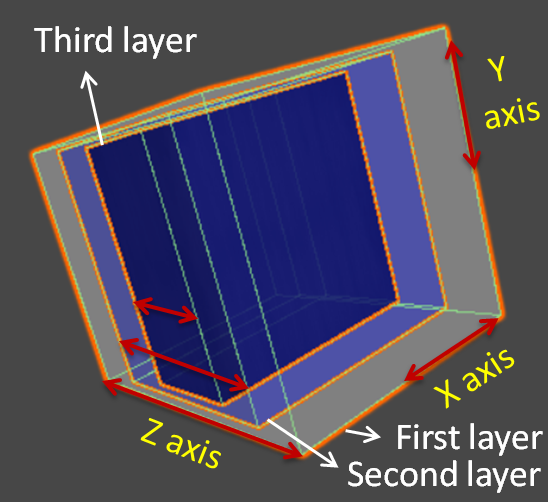
\includegraphics[width=0.3\linewidth]{capitulos/figuras/First.Experiment - axis.PNG} & 
        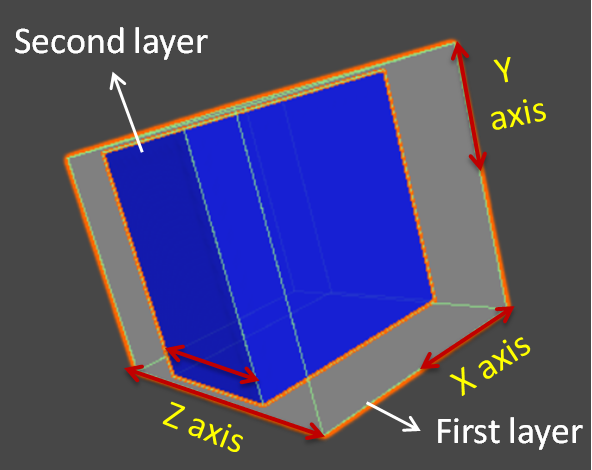
\includegraphics[width=0.35\linewidth]{capitulos/figuras/Second.Experiment - axis.PNG} 
        \\
        (a) & (b)
        \end{tabular}
    \caption{Os objetos 3D representam as camadas de cada experimento: (a) Primeiro experimento (b) Segundo experimento.}
    \label{fig:objectsExperiments}
\end{figure}

O tamanho da agulha é 65 milímetros (mm). Para os dois experimentos foi incluída uma deformação na interface de cada camada com o aumento da força antes da perfuração. Essa deformação é uma função da força necessária para perfurar cada camada. Foi usado um valor máximo de deformação de cinquenta vezes o valor da propriedade \textit{Pop through} em cada camada. O deslocamento desta deformação máxima é medido em milímetros. Logo após ser perfurado o tecido reassume a posição original (sem deformação). 

A Tabela \ref{tab:propHapticoPrimeiroExperimento} descreve os valores configurados nas propriedades de cada camada do primeiro experimento. A deformação máxima para a primeira camada é de 2,5 mm, que corresponde a cinquenta vezes 0,05 (\textit{Pop Through} da primeira camada). A Figura \ref{fig:forcaDeslocamentoExperimento1} apresenta um gráfico da força aplicada (eixo vertical) com o deslocamento da agulha representado no eixo horizontal para o experimento 1. As setas nesta imagem indicam a extensão da deformação de cada camada, começando na esquerda quando a agulha começa a tocar a camada e termina na direita quando a camada é perfurada. O espaço entre as setas da Figura \ref{fig:forcaDeslocamentoExperimento1} representa quando a agulha está em movimento dentro das camadas. As menores variações no eixo horizontal são observadas sob a área das setas por conta da necessidade do aumento de força para se perfurar a camada. As diferenças mais significativas no eixo de deslocamento podem ser observados a direita das setas, marcados com retângulos, que representa o aumento da velocidade de deslocamento da agulha imediatamente após a perfuração da camada.

\begin{table}[!ht]
\begin{center}
\caption{Configurações das propriedade do \textit{plugin} do háptico usadas no primeiro experimento.}
\label{tab:propHapticoPrimeiroExperimento}
\begin{tabular}{|l|lll|}
\hline
\multicolumn{1}{|c|}{\multirow{2}{*}{Propriedade}} & \multicolumn{3}{c|}{Camada}  \\ \cline{2-4} 
\multicolumn{1}{|c|}{} & \multicolumn{1}{c|}{1} & \multicolumn{1}{c|}
{
\begin{tabular}[c]{@{}c@{}}2\end{tabular}} & \multicolumn{1}{c|}{\begin{tabular}[c]{@{}c@{}}3\end{tabular}}  \\ 
\hline\hline
\textit{Stiffness} & \multicolumn{1}{l|}{0,75} & \multicolumn{1}{l|}{0,75} & \multicolumn{1}{l|}{0,75} \\ 
\textit{Pop Through} & \multicolumn{1}{l|}{0,05} & \multicolumn{1}{l|}{0,15} & \multicolumn{1}{l|}{0,10}  \\ 
\textit{Punctured Static Friction} & \multicolumn{1}{l|}{0,20} & \multicolumn{1}{l|}{0,30} & \multicolumn{1}{l|}{0,30}  \\ 
\textit{Punctured Dynamic Friction} & \multicolumn{1}{l|}{0,30} & \multicolumn{1}{l|}{0,30} & \multicolumn{1}{l|}{0,10}  \\ 
\hline
\end{tabular}
\end{center}
\end{table}

O segundo experimento tem duas camadas e sua configuração está descrita na Tabela \ref{tab:propHapticoSegundoExperimento}. A curva de força versus deslocamento da agulha desse experimento está ilustrada na Figura \ref{fig:forcaDeslocamentoExperimento2} e aqui se aplicam as mesmas considerações feitas em relação as marcações de setas e retângulos discutidas em relação a Figura \ref{fig:forcaDeslocamentoExperimento1}.

O ponto de referência que foi considerado para a interface da primeira camada em cada experimento foi 0 mm. Esta referência serve para medir o deslocamento da agulha a partir do toque na primeira camada até atingir todas as demais camadas. Este medida é feita na direção ortogonal da superfície da camada tocada pelo usuário com a agulha virtual. A segunda camada do primeiro experimento está posicionada a 25 mm a partir desta referência e a terceira camada está a 50 mm. A segunda camada do segundo experimento inicia a 35mm do ponto de referência.

\begin{figure}[ht!]
    \centering
    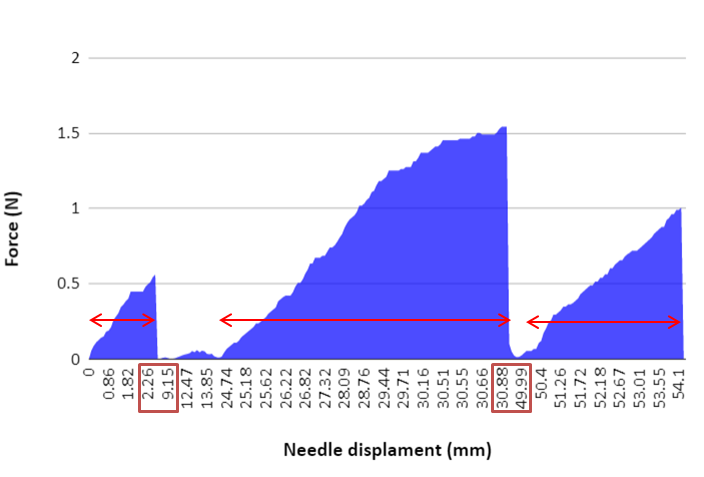
\includegraphics[width=0.8\linewidth]{capitulos/figuras/Experiment 1 - Force x Needle displacement - marked.PNG} 
    \caption{Relação entre força e o deslocamento da agulha da média de dez simulações no experimento 1.}
    \label{fig:forcaDeslocamentoExperimento1}
\end{figure}

\begin{table}[!ht]
\begin{center}
\caption{Configurações das propriedade do \textit{plugin} do háptico usadas no segundo experimento.}
\label{tab:propHapticoSegundoExperimento}
\begin{tabular}{|l|ll|}
\hline
\multicolumn{1}{|c|}{\multirow{2}{*}{Propriedade}} & \multicolumn{2}{c|}{Camada}  \\ \cline{2-3} 
\multicolumn{1}{|c|}{} & \multicolumn{1}{c|}{1} & \multicolumn{1}{c|}{\begin{tabular}[c]{@{}c@{}}2\end{tabular}}  \\  
\hline\hline
\textit{Stiffness} & \multicolumn{1}{l|}{0,75} & \multicolumn{1}{l|}{0,20}  \\ 
\textit{Pop Through} & \multicolumn{1}{l|}{0,05} & \multicolumn{1}{l|}{0,15}  \\ 
\textit{Punctured Static Friction} & \multicolumn{1}{l|}{0,90} & \multicolumn{1}{l|}{0,10}  \\ 
\textit{Punctured Dynamic Friction} & \multicolumn{1}{l|}{0,20} & \multicolumn{1}{l|}{0,10}   \\ 
\hline
\end{tabular}
\end{center}
\end{table}

\begin{figure}[ht!]
    \centering
    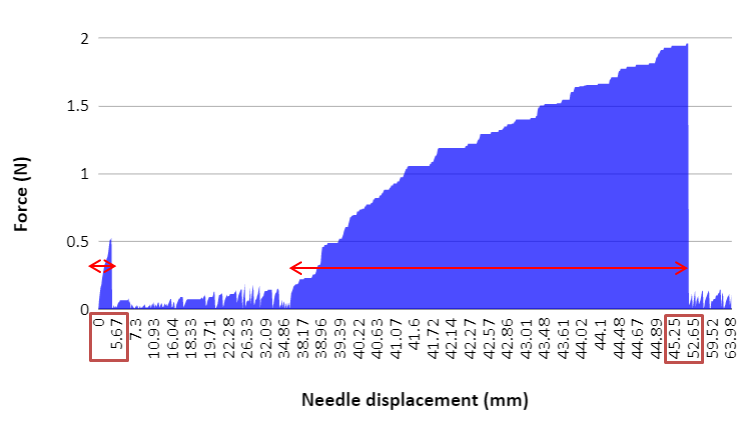
\includegraphics[width=0.8\linewidth]{capitulos/figuras/Experiment 2 - Force x Needle displacement - marked.PNG} 
    \caption{Relação entre força e o deslocamento da agulha da média de dez simulações no experimento 2.}
    \label{fig:forcaDeslocamentoExperimento2}
\end{figure}

A quantidade de camadas de cada experimento proposto aqui difere do número original de camadas do procedimento descrito na seção~\ref{sec:anestesiaRaquidiana}. Isto por que a ideia aqui não é representar todo o corpo ou procedimento. A ideia foi a de reproduzir, nos experimentos, as mais críticas e desafiadoras sensações envolvidas neste procedimento. As outras interfaces entre as camadas são simples reproduções de partes das que foram incluídas nestes experimentos.

\section{Questionário}
\label{sec:questionario}

Após o tempo de testes com a ferramenta de nivelamento no uso do háptico e antes do início do tempo do experimento os questionários com as perguntas de cada experimento foram apresentados para os usuários. Isto foi feito de forma que durante o experimentos cada um pudesse coletar as informações necessárias para responder cada pergunta. Apresentamos a seguir as perguntas dos questionários que foram apresentadas para os voluntários.

Questão 1) Experimentos número 1 e 2: Quantas camadas você pode sentir desde o momento de perfurar o objeto até chegar ao deslocamento máximo de 65mm? 
Observação: Cada camada é identificada por uma restrição a perfuração.

Questão 2) Experimento número 1: Ordene as camadas de forma decrescente em relação a resistência a perfuração.    
Exemplo de resposta: 1, 2 (considerando que existam duas camadas e a primeira é mais resistente que a segunda).

Questão 3) Experimento número 1: Em qual posição cada camada começa, ou seja, qual o ponto do deslocamento da agulha onde você identificou resistência para perfuração? 
Exemplo de resposta: Camada 1 = 0mm, Camada 2 = 10mm e Camada 3 = 30mm (considerando que tenham sido identificadas 3 camadas com resistências nestes 3 pontos de deslocamento).

Questão 4) Experimento número 2: Em qual intervalo (início e fim) de deslocamento foi observado a maior resistência ao movimento de perfuração? 
Exemplo de resposta: Entre 10mm e 20mm.

Questão 5) Experimento número 2: Em qual intervalo (início e fim) de deslocamento foi observado uma necessidade de aplicação de uma força constante para o deslocamento? 
Exemplo: Entre 10mm e 20mm.

Todas as perguntas envolvem aspectos de identificação tátil vitais na realização de uma raquianestesia. Os exemplos de resposta foram ilustrados com o intuito de facilitar a posterior análise das respostas procurando evitar excessos de descrições desnecessárias. A identificação do comportamento elástico é avaliado nas questões 1, 3 e 5 enquanto a questão 4 trata da identificação do comportamento plástico. A questão que envolve a identificação da posição inicial (3) e as que pedem a identificação de intervalos de comportamentos (4 e 5) avaliam a sensação de deformação de cada camada. Todas as camadas iniciam na sua posição de origem e possuem uma deformação imediatamente antes da perfuração que deslocam esta posição. Para fins de avaliação, consideramos corretas as respostas entre o ponto inicial e o ponto final de deformação nas identificações de interface de cada camada.  

\section{Respostas}
\label{sec:respostas}

Nesta seção apresentamos uma compilação das respostas dos participantes às perguntas de cada experimento. Para o primeiro
experimento, as respostas foram as seguintes:

Questão 1) Onze voluntários (aproximadamente 92\%) responderam corretamente.

Questão 2) Sete voluntários (58\%) responderam corretamente para todas as camadas. Onze voluntários (92\%) acertaram a camada menos resistente e nove (75\%) acertaram a mais resistente.

Questão 3) Nove voluntários (75\%) responderam corretamente para todas as camadas. Todos acertaram a segunda camada e onze voluntários (92\%) acertaram a primeira camada.

Após responder o primeiro questionário as mesmas pessoas executaram o segundo experimento e responderam o questionário deste conforme descrito a seguir:

Questão 1) Todos os voluntários (100\%) responderam corretamente.

Questão 4) Nove voluntários (75\%) responderam corretamente.

Questão 5) Cinco voluntários (42\%) responderam corretamente. Nove (75\%) acertaram o início.

\section{Avaliação dos resultados}
\label{sec:avaliacao}

Nesta seção detalhamos cada um dos comportamentos mais importantes do procedimento coberto nestes experimentos que foram criados para avaliar a percepção do usuário sobre o comportamento das
camadas virtuais sendo perfuradas por uma agulha.

\subsection{Resistência à punção}

Considerando os sentimentos ou sensações resistência à punção (o assunto da questão dois), apenas 58\% dos respondentes ordenaram corretamente todas as camadas de acordo com suas resistências. Este resultado indica a necessidade de se aumentar a diferença na força necessária para perfurar cada camada para permitir uma identificação mais facilitada de todas estas características. Na mesma pergunta, um número maior de voluntários identificaram a camada mais resistente ou a menos resistente à perfuração. Essa identificação é essencial para indicar quando a agulha penetra no ligamento amarelo (tecido mais resistente) ou a dura-máter (tecido menos resistente). Como estas duas camadas estão posicionadas no corpo humano uma após a outra (considerando o ângulo de perfuração correto), a correta identificação de uma é, por si só, um passo essencial na simulação correta do procedimento de raquianestesia.

\subsection{Comportamento elástico}

Quanto à identificação do comportamento elástico (questões 1, 3 e 5), apenas a questão cinco recebeu pontuação inferior a 75\%. No entanto, mesmo nesta questão, apenas três voluntários apontaram erroneamente o ponto de partida do intervalo com maior restrição ao movimento da agulha. Assim, quase todos os participantes puderam apontar onde esta camada começa. No entanto, o mesmo resultado não foi alcançado na identificação do seu fim, com mais da metade (58\%) perdendo o ponto final. Analisando as respostas e o modelo, a causa mais provável disso indica que o curva utilizada foi muito alta, pois houve uma queda significativa na pressão e grande deslocamento da agulha quando o usuário deixou este camada. Assim, se identificar o final da camada é essencial para o problema, é necessário reduzir a queda de pressão no modelo para melhor simular esse comportamento.

Tivemos ótimas respostas na detecção do número de camadas (questão um) em todos experimentos. Identificar as camadas penetradas é uma das partes mais críticas do procedimento de raquianestesia. Isto indica tanto a determinação correta da sensação de \textit{popping} da interface entre as camadas e reconhecimento do comportamento elástico que ocorre imediatamente antes de perfurar cada camada.

Quanto à identificação do ponto de início de cada camada, o assunto da questão três, também é importante destacar o número de casos corretamente identificados (75\%). Esta resposta reforça a necessidade de utilização de valores de profundidade desde a pele até o espaço subaracnóide próximo da realidade para treinar melhor os anestesistas. Cada ponto de partida da camada está relacionado com o início do comportamento elástico e é necessário aumentar a força para prosseguir com o avanço da agulha em cada interface entre camadas.

\subsection{Comportamento plástico}

A questão quatro, com 75\% de sucesso na identificação, aborda um outro comportamento de grande importância na raquianestesia. A identificação de estar dentro da camada que apresenta a maior
resistência, ou seja, sentir uma pressão constante contra o movimento através da camada (comportamento plástico), está relacionado ao ligamento amarelo, que ocorre imediatamente antes de se atingir o espaço peridural. As respostas a esta pergunta
confirmam que esse comportamento pode ser simulado adequadamente.